\section{Exercise 4: Dale's law}

\begin{itshape}
\small
Set $c=0.1$, $N = 200$ and turn off random asymmetry ($p_{cut} = 0$). Set $E \in \l[0, 1\r]$ to be the percentage of excitatory nodes.

For a given $E$, randomly split the network into an excitatory and an inhibitory subpopulation (of sizes $E \cdot N$ and $(1 - E) \cdot N$ respectively). Now enforce Dale's law on the network connectivity by setting "disallowed" connection weights in the standard Hebbian weight matrix Eq. 1 to zero.

What percentage of the directed connections do you expect to be cut for $E = \frac{1}{2}$
As in Ex. 2 calculate and plot the mean $\alpha_{N,max}$ for varying E with error bars (at least 10 repetitions). Interpret the results and compare the value for E$ = 1$ to your result from Ex. 3.
\end{itshape}

\paragraph*{}

As a reminder we restate Dale's law; \textit{for each neuron, synaptic connections to postsynaptic neurons are either of the excitatory or inhibitory type, never both} (Exercise Sheet).

\begin{figure}[H]
  \begin{center}
    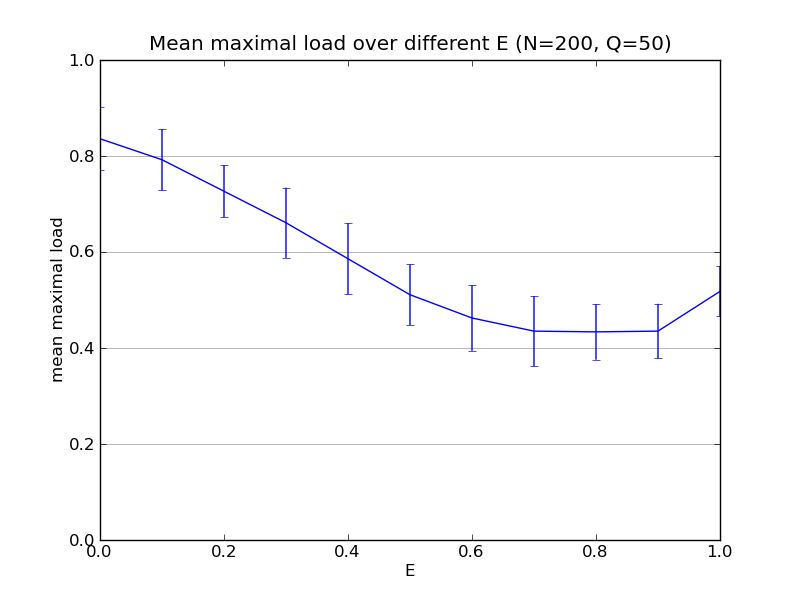
\includegraphics[width=0.6\textwidth]{dat/ex4-mean_max_load-N200-Q50-C95.png}
  \end{center}
  \vspace{-20pt}
  \caption{Exercise 4: Mean maximal load over different E}
  \label{fig: exercise 4}
\end{figure}

\paragraph*{}
When E increases from 0 to 0.7, the mean maximal load decreases. After 0.7 it flattens out and then starts increasing again just before E $= 1$. E $=1$ means that all nodes are excitatory and therefore all weights positive as can be deduced from equation \ref{eq: weights}. As shown in figure \ref{fig: exercise 4}, we expect the mean maximal load to decrease as E increases. 

Expecting all patterns $\xi_i$ being uniformly random and the weight matrix symmetric we expect for all $E$ and so for $E = \frac{1}{2}$ half the nodes to be cut.
So the maximal available load should be $\alpha_{N,max} = 0.08$. 

But we find that is for E $= 0$ $\alpha_{N,max} = 0.10 $. Indeed we receive with this kind of weight cutting better results than with random weight cutting with $P_cut=0.5$  for $E \in [0 \ldots 0.4] $. For higher excitatory nodes parts (shares? anteile) we fall below these values. For E $ = 1$ the value (0.07) is bit lower than the random cut  value (0.075).

This shows that a high excitatory (anteil) is worse than a random cut in same size but for low excitatory (anteile) it is better. So even if in more-realistic Hopfield neuron models Dale's Law is enforced and therefore weights are cut, it can better recover a random pattern.


	